\begin{Soln}{2}
On obtient un triangle équilatéral.
\end{Soln}
\begin{Soln}{3}
Considérer la symétrie axiale d'axe $(AC)$.
On note $B'$ l'image de $B$ par cette symétrie.
Ensuite, projeter perpendiculairement le point $B$ sur la droite $(AB')$, et reconnaître un triangle rectangle ayant un angle de $30^\circ$ et une hypoténuse de $1cm$.
\end{Soln}
\begin{Soln}{5}
Complétons la figure comme suit :
\begin{center}
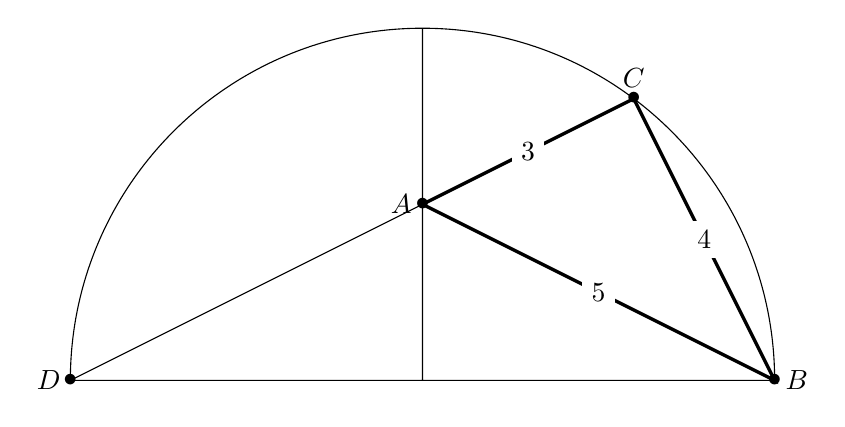
\begin{tikzpicture}[scale=1]
\draw (0,0) -- ({2*sqrt(5)},0) arc (0:180:{2*sqrt(5)}) node[left] {$D$} node {$\bullet$} -- (0,0) -- (0,{2*sqrt(5)});
\draw[very thick] (0,{sqrt(5)}) node {$\bullet$} node[left] {$A$}
-- ({2*sqrt(5)},0) node[midway,fill=white] {$5$} node {$\bullet$} node[right] {$B$}
-- ({3*2*sqrt(5)/5},{sqrt(5)+3/sqrt(5)}) node[midway,fill=white] {$4$} node {$\bullet$} node[above] {$C$}
-- cycle node[midway,fill=white] {$3$}  ;
\draw ({-2*sqrt(5)},0)-- (0,{sqrt(5)});
\end{tikzpicture}
\end{center}
Comme le triangle $ABC$ est rectangle en $C$, la droite $(AC)$ recoupe le droite $(OB)$ en $D$. Le triangle $DBC$ est rectangle en $C$ et on a $DC=8$ et $BC=4$, donc en appliquant le théorème de Pythagore, on obtient
\[ DB=\sqrt{64+16}=\sqrt{80} = 4\sqrt5.\]
Le rayon est donc égal à $2\sqrt 5$.
\end{Soln}
\begin{Soln}{6}
Pour le deuxième carré, on a intérêt à noter $60x$ le côté du carré, de cette façon c'est divisible par $3$, $4$ et $5$. Ensuite on utilise les triangles semblables, mais du coup cet exo est faisable sans Pythagore. On trouve que $x=\frac{1}{37}$ par proportionnalité, le deuxième carré fait donc $60/37$ de côté.

Avec Pythagore ça doit être plus pénible...

Le première carré fait $12/7$ de côté. Là aussi, on a intérêt à noter $12y$ le côté, comme ça c'est divisible par trois et quatre. Et là aussi il vaut mieux faire ça avec des triangles semblables.
Il est plus gros que le premier car $444=12\times 37 \geq 7\times 60=420$. Sur le dessin ça se voir quand même assez nettement.
\end{Soln}
\begin{Soln}{7}
En appliquant le théorème de Pythagore, on voit que les deux aires sont égales  à $\dfrac 45 R^2$ !
\end{Soln}
\begin{Soln}{8}
On trouve une hauteur de $12$, et un rayon de $\frac{169}{24}$.
\end{Soln}
\begin{Soln}{9}
On peut par exemple projeter le centre du rectangle sur une base, noter $x$ la distance de $O$ à ce projeté, et on obtient alors en considérant la largeur et la hauteur du rectangle :  $3=2R+2x$ et $2=2\sqrt{R^2-x^2}$, c'est-à-dire $1=R^2-x^2=\frac32(R-x)$, d'où finalement le système $R+x=\frac32$ et $R-x=\frac23$ et donc $2R=\frac{9+4}{6}$ et finalement $R=\frac{13}{12}$.

Autre méthode : on projette $O'$ sur la base, et on applique Pythagore dans $OO'H$. On a $OH=3-2R$, donc :
\[ (3-2R)^2+4=4R^2\]
Et donc $13-12R=0$, c'est plus rapide !
\end{Soln}
\begin{Soln}{11}
Les triangles $ADP$ et $AQB$ sont égaux : ils ont les mêmes angles et la même hypoténuse.
On en déduit que $AP=4$ et $AQ=5$, et en appliquant le théorème de Pythagore, on trouve le côté du carré : $AB=\sqrt{41}$.
Le carré a donc une aire de $41\mathrm{cm}^2$.

Pour trouver la distance $AM$, il suffit de trouver $QM$. Le plus simple est d'utiliser des triangles semblables, ou Thalès, on trouve $QM=16/5$, donc $AM=5+16/5=41/5$.
\end{Soln}
\begin{Soln}{12}
Le rayon du quart de cercle est $\sqrt 3$.
\end{Soln}
\begin{Soln}{13}
\end{Soln}
\begin{Soln}{16}
On fait Pythagore dans les trois triangles et ça se simplifie.

Évidemment on pourrait faire ça plus joliment avec des triangles semblables.
\end{Soln}
\begin{Soln}{17}
En calculant l'aire du triangle de deux façons, on a $AH\times BC = AB\times AC$.

Ensuite, on peut procéder de plusieurs façons, juste avec Pythagore dans les trois triangles rectangles, ou en remarquant des triangles semblables.
Par exemple, comme $ABH$ et $CAH$ sont semblables, on a, par proportionnalité, le produit en croix $AH^2=HB\times HC = 16 HB$.

Ensuite, en appliquant le théorème de Pythagore dans le triangle $ABH$ rectangle en $H$, on obtient:
\[ 15^2 = AH^2+BH^2 = 16BH+BH^2 = (BH+8)^2-64\]
On en tire $BH+8=\sqrt{15^2+8^2}=\sqrt{289}=17$, d'où $BH=17-8=9$.

Ensuite, on continue et on trouve normalement $AH=12$ et $AC=20$.
\end{Soln}
\begin{Soln}{19}
Source : \url{https://twitter.com/Math_World_/status/1519662926860365824}

On peut utiliser le théorème de la hauteur relative à l'hypoténuse (citer référence du problème).

On peut aussi refaire trois fois Pythagore, (ou bien utiliser les triangles semblables, ou utiliser la puissance du point $K$ par rapport au cercle.)
\end{Soln}
\begin{Soln}{20}
On a
\[
A^2 = 11+6\sqrt 2 = 11+\sqrt{72},\quad
B^2 = 11+2\sqrt{30}=11+\sqrt{120} \quad\text{et}
C^2 = 11+2\sqrt{10}=11+\sqrt{40}.\]
On en déduit que
\[ C< A < B.\]
\end{Soln}
\begin{Soln}{23}
Le diamètre est $5$.
\end{Soln}
\begin{Soln}{24}
Le rayon vaut $\sqrt{85}/4$.
\end{Soln}
\begin{Soln}{25}
Le côté vaut $\sqrt{10}$.

Pour le second la source d'origine est : \url{https://twitter.com/0y6tr4/status/1522092641017602049}. Mais en fai le premier est mieux, plus simple
\end{Soln}
\begin{Soln}{26}
On obtient $AB=\sqrt 6 + 2\sqrt 6 = 3\sqrt 6$. (on fait deux fois Pythagore)
\url{https://twitter.com/0y6tr4/status/1521866673493618690}
\end{Soln}
\begin{Soln}{27}
\url{https://erich-friedman.github.io/packing/cirinsqu/}
VERIFIER Le carré est de côté $2+\frac{1}{\sqrt 2} + \frac{\sqrt 6}{2}$.

Pour le premier le côté vaut $2+\sqrt2$.
\end{Soln}
\begin{Soln}{28}
Le carré a un côté de $2+\frac{12}{\sqrt 13}$. Voir la vidéo \url{https://www.youtube.com/watch?v=ONs1u3xRzrM&t=12s} et bien sûr le site \url{https://erich-friedman.github.io/packing/cirinsqu/}.
\end{Soln}
\begin{Soln}{29}
\url{https://erich-friedman.github.io/packing/squinsqu/}
\end{Soln}
\begin{Soln}{30}
\url{https://erich-friedman.github.io/packing/squinsqu/}
\end{Soln}
\begin{Soln}{31}
\end{Soln}
\begin{Soln}{33}
On a
\[
A^2 = 11+6\sqrt 2 = 11+\sqrt{72},\quad
B^2 = 11+2\sqrt{30}=11+\sqrt{120} \quad\text{et}
C^2 = 11+2\sqrt{10}=11+\sqrt{40}.\]
On en déduit que
\[ C< A < B.\]
\end{Soln}
